\documentclass[11pt,preprint, authoryear]{elsarticle}

\usepackage{lmodern}
%%%% My spacing
\usepackage{setspace}
\setstretch{1.2}
\DeclareMathSizes{12}{14}{10}{10}

% Wrap around which gives all figures included the [H] command, or places it "here". This can be tedious to code in Rmarkdown.
\usepackage{float}
\let\origfigure\figure
\let\endorigfigure\endfigure
\renewenvironment{figure}[1][2] {
    \expandafter\origfigure\expandafter[H]
} {
    \endorigfigure
}

\let\origtable\table
\let\endorigtable\endtable
\renewenvironment{table}[1][2] {
    \expandafter\origtable\expandafter[H]
} {
    \endorigtable
}


\usepackage{ifxetex,ifluatex}
\usepackage{fixltx2e} % provides \textsubscript
\ifnum 0\ifxetex 1\fi\ifluatex 1\fi=0 % if pdftex
  \usepackage[T1]{fontenc}
  \usepackage[utf8]{inputenc}
\else % if luatex or xelatex
  \ifxetex
    \usepackage{mathspec}
    \usepackage{xltxtra,xunicode}
  \else
    \usepackage{fontspec}
  \fi
  \defaultfontfeatures{Mapping=tex-text,Scale=MatchLowercase}
  \newcommand{\euro}{€}
\fi

\usepackage{amssymb, amsmath, amsthm, amsfonts}

\def\bibsection{\section*{References}} %%% Make "References" appear before bibliography


\usepackage[round]{natbib}

\usepackage{longtable}
\usepackage[margin=2.3cm,bottom=2cm,top=2.5cm, includefoot]{geometry}
\usepackage{fancyhdr}
\usepackage[bottom, hang, flushmargin]{footmisc}
\usepackage{graphicx}
\numberwithin{equation}{section}
\numberwithin{figure}{section}
\numberwithin{table}{section}
\setlength{\parindent}{0cm}
\setlength{\parskip}{1.3ex plus 0.5ex minus 0.3ex}
\usepackage{textcomp}
\renewcommand{\headrulewidth}{0.2pt}
\renewcommand{\footrulewidth}{0.3pt}

\usepackage{array}
\newcolumntype{x}[1]{>{\centering\arraybackslash\hspace{0pt}}p{#1}}

%%%%  Remove the "preprint submitted to" part. Don't worry about this either, it just looks better without it:
\makeatletter
\def\ps@pprintTitle{%
  \let\@oddhead\@empty
  \let\@evenhead\@empty
  \let\@oddfoot\@empty
  \let\@evenfoot\@oddfoot
}
\makeatother

 \def\tightlist{} % This allows for subbullets!

\usepackage{hyperref}
\hypersetup{breaklinks=true,
            bookmarks=true,
            colorlinks=true,
            citecolor=blue,
            urlcolor=blue,
            linkcolor=blue,
            pdfborder={0 0 0}}


% The following packages allow huxtable to work:
\usepackage{siunitx}
\usepackage{multirow}
\usepackage{hhline}
\usepackage{calc}
\usepackage{tabularx}
\usepackage{booktabs}
\usepackage{caption}


\newenvironment{columns}[1][]{}{}

\newenvironment{column}[1]{\begin{minipage}{#1}\ignorespaces}{%
\end{minipage}
\ifhmode\unskip\fi
\aftergroup\useignorespacesandallpars}

\def\useignorespacesandallpars#1\ignorespaces\fi{%
#1\fi\ignorespacesandallpars}

\makeatletter
\def\ignorespacesandallpars{%
  \@ifnextchar\par
    {\expandafter\ignorespacesandallpars\@gobble}%
    {}%
}
\makeatother

\newenvironment{CSLReferences}[2]{%
}

\urlstyle{same}  % don't use monospace font for urls
\setlength{\parindent}{0pt}
\setlength{\parskip}{6pt plus 2pt minus 1pt}
\setlength{\emergencystretch}{3em}  % prevent overfull lines
\setcounter{secnumdepth}{5}

%%% Use protect on footnotes to avoid problems with footnotes in titles
\let\rmarkdownfootnote\footnote%
\def\footnote{\protect\rmarkdownfootnote}
\IfFileExists{upquote.sty}{\usepackage{upquote}}{}

%%% Include extra packages specified by user

%%% Hard setting column skips for reports - this ensures greater consistency and control over the length settings in the document.
%% page layout
%% paragraphs
\setlength{\baselineskip}{12pt plus 0pt minus 0pt}
\setlength{\parskip}{12pt plus 0pt minus 0pt}
\setlength{\parindent}{0pt plus 0pt minus 0pt}
%% floats
\setlength{\floatsep}{12pt plus 0 pt minus 0pt}
\setlength{\textfloatsep}{20pt plus 0pt minus 0pt}
\setlength{\intextsep}{14pt plus 0pt minus 0pt}
\setlength{\dbltextfloatsep}{20pt plus 0pt minus 0pt}
\setlength{\dblfloatsep}{14pt plus 0pt minus 0pt}
%% maths
\setlength{\abovedisplayskip}{12pt plus 0pt minus 0pt}
\setlength{\belowdisplayskip}{12pt plus 0pt minus 0pt}
%% lists
\setlength{\topsep}{10pt plus 0pt minus 0pt}
\setlength{\partopsep}{3pt plus 0pt minus 0pt}
\setlength{\itemsep}{5pt plus 0pt minus 0pt}
\setlength{\labelsep}{8mm plus 0mm minus 0mm}
\setlength{\parsep}{\the\parskip}
\setlength{\listparindent}{\the\parindent}
%% verbatim
\setlength{\fboxsep}{5pt plus 0pt minus 0pt}



\begin{document}



\begin{frontmatter}  %

\title{Baby Names in the US}

% Set to FALSE if wanting to remove title (for submission)




\author[Add1]{Anna Mayer}
\ead{28776534@sun.ac.za}





\address[Add1]{Stellenbosch University}


\begin{abstract}
\small{
Analysis of past and current trends in baby names in the US and factors
that influenced choices over time.
}
\end{abstract}

\vspace{1cm}


\begin{keyword}
\footnotesize{
Baby Names \\
\vspace{0.3cm}
}
\end{keyword}



\vspace{0.5cm}

\end{frontmatter}

\setcounter{footnote}{0}



%________________________
% Header and Footers
%%%%%%%%%%%%%%%%%%%%%%%%%%%%%%%%%
\pagestyle{fancy}
\chead{}
\rhead{}
\lfoot{}
\rfoot{\footnotesize Page \thepage}
\lhead{}
%\rfoot{\footnotesize Page \thepage } % "e.g. Page 2"
\cfoot{}

%\setlength\headheight{30pt}
%%%%%%%%%%%%%%%%%%%%%%%%%%%%%%%%%
%________________________

\headsep 35pt % So that header does not go over title




\hypertarget{introduction}{%
\section{\texorpdfstring{Introduction
\label{Introduction}}{Introduction }}\label{introduction}}

This analysis focuses on baby name trends, how they persist over time
and which factors are influencing parents decision in naming their
children across the past decades.

\hypertarget{data}{%
\section{Data}\label{data}}

The data used for this analysis is mainly a list of baby names form 1910
to 2014. Moreover, for the factor analysis, a closer look was taken into
data on HBO titles and charts.

\hypertarget{analysis}{%
\section{Analysis}\label{analysis}}

Firstly, this report tried to determine how well popular names persist
into the future using the Spearman rank correlation. More
specifically,the Spearman rank correlation of the top 25 boys' and
girls' names for each year with the subsequent three years was
calculated and then plotted in \ref{Figure1} below.

\begin{figure}[H]

{\centering \includegraphics{Question1_files/figure-latex/Figure1-1} 

}

\caption{Persistence of Baby Names over Time \label{Figure1}}\label{fig:Figure1}
\end{figure}

Note that the scale on the y-axis ranges from 0.5 to 1.

Especially in the 1960s, female names do not seem to be correlated.
However, until 1950, there seems to be a correlation for both male and
female baby names. In general, there seems to be a slight downward
trend, meaning that past 3 years baby names do not seem to be as
positively correlated as in the beginning of the 20th century.
Nevertheless, the coefficient is still relatively high for both genders.
One can conclude from this graph, that popular baby names still persist
until today, although there is a small downward trend. As mentioned, the
reason for this is that the average correlation coefficient (averaged
for following 3 years) is still high even after 1990 for both genders.
Given the long-term trend, one can expect this persistence with a
potentially continuing very small downward trend for the future.

In a next step, this report focuses on factors influencing the choice of
baby names. For this, please find below the year-on-year percentage
change for the three names Krystle, Khaleesi and Neymar:

\begin{figure}[H]

{\centering 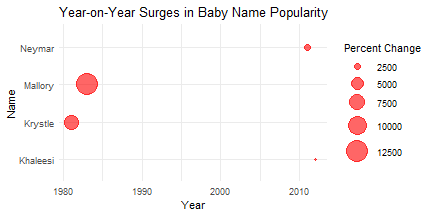
\includegraphics{Question1_files/figure-latex/Figure2-1} 

}

\caption{Surges in Baby Names \label{Figure2}}\label{fig:Figure2}
\end{figure}

Interestingly, in 2012, there was an increase of 2010 \% of the name
Khaleesi (from 5 to 110). This is most likely related to Game of Thrones
(which was according to the HBO\_Titles data set released in 2011). Game
of Thrones, with an audience popularity score of 492.101 became very
famous very quickly and probably influenced the naming decisions of many
parents. Moreover, looking at the surges data, one can see that in 2011,
the name Neymar experienced an increase of 2700\%, which might be
related to Neymar's starting his professional soccer career back in 2009
(Caioli (\protect\hyperlink{ref-caioli2017neymar}{2017})).In 1981,
Krystle got a spike with 6816 \%. This is most likely related to Krystle
Carrington, a fictional character from the 1980s American TV series
Dynasty. Also Mallory experienced a strong increase in the 1983 which is
probably related to the sitcom Family Ties and one of the main
characters names Mallory Keaton in 1982.

From this, one can see, that different factors influence baby names,
from soccer players to sitcoms to movies or tv-shows.

\hypertarget{conclusion}{%
\section{Conclusion}\label{conclusion}}

There is persistence over time in baby names, which could be clearly
seen in \ref{Figure1}.Therefore, sticking to classical popular baby
names like Mary, James, Lisa, etc. might be a good idea for toys.
However, there are also factors that lead to spikes in the appearance of
more unusual baby names such as Khaleesi, Krystle, Neymar etc. This
could be taken into account. Current, popular TV shows, soccer players
etc. influence the choice of parents with respect to naming their babies
and therefore could also serve as good names for toys. However, this
comes with the cost of changing toys names once in a while, as trends
are changing with new tv shows and people becoming famous.

For further research on traditional, persisting names, one could have a
closer look into bible names data, for example using Hitchcock's Bible
Names Dictionary. Since religion probably still influence the decision
of many parents in naming their children. A list and analysis can be
provided on request from me.

\newpage

\hypertarget{references}{%
\section*{References}\label{references}}
\addcontentsline{toc}{section}{References}

\hypertarget{refs}{}
\begin{CSLReferences}{1}{0}
\leavevmode\vadjust pre{\hypertarget{ref-caioli2017neymar}{}}%
Caioli, L. 2017. \emph{Neymar--2018 updated edition: The unstoppable
rise of barcelona's brazilian superstar}. Icon Books.

\end{CSLReferences}

\bibliography{Tex/ref}





\end{document}
